\documentclass[a4paper,10pt]{article}

%%
%% CadenceLIVE Template
\usepackage[left=25mm,right=25mm,top=20mm,bottom=20mm]{geometry}
\usepackage{authblk}
\usepackage[T1]{fontenc}
\usepackage{helvet}
\usepackage{graphicx}
\usepackage{nopageno}
\usepackage{parskip}
\usepackage{titlesec}
\usepackage{etoolbox}
\usepackage{soul}

%%
%% Arial Font config
\renewcommand{\sfdefault}{phv}
\renewcommand{\familydefault}{\sfdefault}

%%
%% Author Block
\renewcommand*{\Authsep}{, }
\renewcommand*{\Authand}{, }
\renewcommand*{\Authands}{, }
\renewcommand*{\Authfont}{}
\renewcommand*{\Affilfont}{}
\setlength{\affilsep}{6pt}

%%
%% Title Block
\newcommand{\logo}{./fig/cadencelive-2022.pdf}

\makeatletter
\renewcommand{\maketitle}{%
\vspace*{-0.5cm}
\includegraphics[width=0.32\textwidth]{\logo}
\vspace{35pt}
\begin{center}
    {\LARGE\noindent\ignorespaces\bfseries\@title\par}
    \linespread{1.5}
    \vspace{10pt}
    {\large\noindent\ignorespaces\@author\par}
    %{\normalsize\noindent\ignorespaces\@affil\par}
	{\large\noindent\ignorespaces\email\par}
    \linespread{1.0}
\end{center}}
\makeatother

%%
%% Abstract
\makeatletter
\renewenvironment{abstract}{%
    \vspace*{5mm}
    \noindent\begin{minipage}{1\textwidth}
    \begin{center}
    \textbf{\fontsize{14}{3}\selectfont Abstract}
    \bigskip
    \end{center}
    \fontsize{12}{3}\selectfont
    \medskip

}{\end{minipage}}
\makeatother

%%
%% Keywords
\makeatletter
\newenvironment{keywords}{%
    \vspace{.5em}
    \noindent\begin{minipage}{1\textwidth}
        \textbf{\fontsize{12}{3}\selectfont Keywords:}\fontsize{10}{3}\selectfont
}{\end{minipage}}
\makeatother

%%
%% Keywords
\makeatletter
\newenvironment{acknowledgment}{%
    \noindent\begin{minipage}{1\textwidth}
    \bigskip
    \section*{Acknowledgments}
}{\end{minipage}}
\makeatother

%%
%% Reformatting Table and Figure lables
\renewcommand{\tablename}{\fontsize{8}{3}\selectfont Tab.}
\renewcommand{\figurename}{\fontsize{8}{3}\selectfont Fig.}
\setlength\abovecaptionskip{2pt}
\setlength\belowcaptionskip{5pt}

%%
%% Section formatting
\titleformat{\section}{\fontsize{12}{6}\selectfont}{\textbf{\thesection .}}{0.5em}{\textbf}
\titlespacing{\section}{0pt}{10pt}{6pt}

%%
%% No paragraph indentation
\setlength{\parindent}{0pt}

%%
%% Bibliography
\makeatletter
\renewenvironment{thebibliography}[1]{%
    \section*{\fontsize{12}{14}\selectfont\refname}%
    \@mkboth{\MakeUppercase\refname}{\MakeUppercase\refname}%
    \list{\@biblabel{\@arabic\c@enumiv}}{%
        \settowidth\labelwidth{\@biblabel{#1}}%
        \leftmargin\labelwidth\advance\leftmargin\labelsep
        \@openbib@code\usecounter{enumiv}\let\p@enumiv\@empty
        \renewcommand\theenumiv{\@arabic\c@enumiv}}\sloppy
        \clubpenalty4000
        \@clubpenalty \clubpenalty
        \widowpenalty4000\sfcode`\.\@m}
        {\def\@noitemerr{\@latex@warning{Empty `thebibliography' environment}%
        }\endlist}
\makeatother


%%
%% Paper Title
\title {Abstract Guidelines for CadenceLIVE Europe 2022 -- Academic Track}

%%
%% Author Block
\author[*]{First Author}
\author[**]{Second Author}
\author[***]{Third Author}
\affil[*]{company, address, town, country}
\affil[**]{company, address, town, country}
\affil[***]{company, address, town, country}
\newcommand{\email}{corresponding author's e-mail address}

\begin{document}

%%
%% Header Formatting and Title
\maketitle

%%
%% Use abstract environment for the abstract
\begin{abstract}
An abstract of maximum 150 – 250 words should be appropriate for this section.
The word "Abstract" should be Arial, 14pt, bolded, initially capitalized, and
centered above the abstract text. The spacing for the word "Abstract": 18pt
before and 12pt after. The text of this section should be single-spaced, Arial,
12pt, non-bolded. Very important, in all the sections the text must be
justified, except where another requirement is clearly specified. The spacing
for this section: 0pt before and 12pt after. 
\end{abstract}

%%
%% Use keywords environment for the keywords
\begin{keywords}
List four to six descriptive words across the page. The spacing for this
section: 0pt before and 12pt after. The word "Keywords" should be Arial, 12pt,
bolded, aligned to left. The text of this section should be Arial, 10pt,
non-bolded.
\end{keywords}

%%
%% Section headings shouldn't be numbered according to the template
\section*{Main Title and Title of Paragraphs (Headings)}

Very important, the two-page abstract must clearly state what is NEW in the
paper with respect to the state of the art. The main title should be easily
readable, Arial, 18pt, bolded, initially capitalized, and centered above the
abstract text. In the main title, do not capitalize articles, coordinate
conjunctions, and prepositions under four letters in length. The main title
should have a spacing of 12pt before the title (between the logo and the title)
and 6pt after. The main title should be followed by the section with the
details of the author(s), Arial, 12pt, centered. Only the names of author(s)
will be bolded. The spacing for this section: 0pt before and 6pt after. 

The titles of paragraphs should be Arial, 12pt, bolded, initially capitalized,
and left-aligned above the paragraph text. Do not capitalize articles,
coordinate conjunctions, and prepositions under four letters in length. The
spacing for titles of paragraphs (headings): 12pt before and 6pt after. 

\section*{Format of Your Abstract}

Use A4 format for your two-page abstract. All printed materials, including
texts, figures, illustrations, tables, and charts must be kept within the
parameters of the one-column format. Left, right, top, and bottom margins
should each be 25mm. Succeeding pages will have a 25mm top margin.
\ul{%
We strongly advise you to use the present document as the official template and
to introduce your text/figures/tables in it.} 
Print out these instructions before
pasting your work into this document, so you can refer back to it. Regarding
the names of paragraphs, we recommend the following: 
\textbf{Introduction and Motivation of Work, Results, Conclusions, Acknowledgements},
and \textbf{References}.

\section*{Type Style and Size}

The text of all sections should be Arial, 10pt, non-bolded, justified. Text
should be single-spaced. The spacing for all sections: 0pt before and 6pt
after. 

\section*{Figures, Graphs, Photographs, and Tables}

The figures, graphs, tables, and photographs may fit with the text, but can be
smaller, if necessary. Figures, graphs, and photographs should be color or B\&W
of high quality, centered on the page. 

Figure, graph, photograph, and table captions should be Arial, 9pt, and
centered but not bolded, as presented below. The spacing for all captions: 3pt
before and 3pt after. The spacing for a a figure, graph, or photograph: 12pt
before and 0pt after. 

\begin{table}[!htb]
    \centering
    \caption{Measurement results}\label{tab:measure}
    \smallskip
        \begin{tabular}{ | c | c | c | c | c | } \hline
            \textbf{Voltage [V]} & \textbf{Current [A]} & \textbf{Frequency [Hz]} 
                & \textbf{Capacitance [nF]} & \textbf{Inductance [mH]} \\ 
            \hline
            1 & 1 & 1 & 1 & 1 \\ 
            \hline 
        \end{tabular}
\end{table}

The caption is placed above the table and below the figure/graph/photograph. As
general rule, each figure/graph/photograph or table should occupy one-fourth to
one-third of a page. 

\begin{figure}[!h]
    \centering
    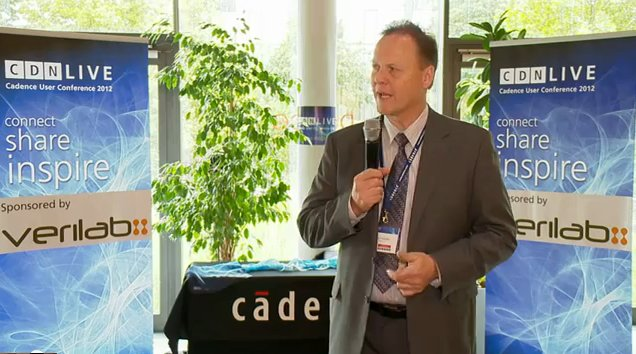
\includegraphics[width=2.3984in,height=1.3437in]{./fig/cadencelive-ceremony.jpg}
    \label{fig:ceremony}
    \caption{CDNLive EMEA 2017 Best PresentationPaper Awards Ceremony}
\end{figure}

\section*{Pagination, Page Limits, and Submission}

Do NOT place page numbers on the manuscript. This will be done by the
publishers. You are asked to limit the abstract to two pages. Papers should be
submitted in Microsoft Word format or Adobe Acrobat PDF format. Please follow
carefully the instructions given in this template. Name the files with the
corresponding author’s last name at the beginning and with "CadenceLIVE2022" at
the end (for example: \textbf{Codreanu\_abstract\_CadenceLIVE2022.doc} and
\textbf{Codreanu\_abstract\_CadenceLIVE2022.pdf}).

\section*{Copyright}

By submitting the paper, the authors accept that Cadence may reproduce,
publish, and distribute the submitted materials in the CadenceLIVE Proceedings
for use by Cadence employees, contractors, and licensees, Cadence may reproduce
and post the submitted materials on the CadenceLIVE website for access by
Cadence employees, contractors, and licensees, Cadence shall reproduce any
copyright or other legal notices that the authors include in the submitted
materials, and Cadence will not use the materials for product marketing
purposes without first obtaining the express written consent of authors. 

%%
%% Use acknowledgment environment for the acknowledgments
\begin{acknowledgment}
Acknowledgments can be placed, if necessary, after conclusions and before the
references list. 
\end{acknowledgment}

%%
%% Bibliography, make sure title is in italics
\begin{thebibliography}{9}
    \bibitem{WHEEL}
    M. Neanderthal, \textit{The Invention of the Wheel}, Proceedings of the 20000 B.C. Paleo-Eelectronic Components and Packaging Conference, Vindija, Croatia, August 12-15, pp. 21-30, 20000 B.C.
    
    \bibitem{UFO}
    N. D. Forester, \textit{Advanced Investigations on Roswell UFO Materials}, Journal of Extra-Tterrestrial Materials, Vol. 3, No. 5, pp. 24-29, November, 2012.
    
    \bibitem{WAYNE}
    J. Wayne, \textit{The Book of My Western Films}, Marion Morrison Publishers, second edition, New York, Chapter 3, pp. 229-243, 1947.
\end{thebibliography}

\end{document}
